\begin{tikzpicture}
  \node[anchor=south west, inner sep=0] (miimage) at (0,0)
    {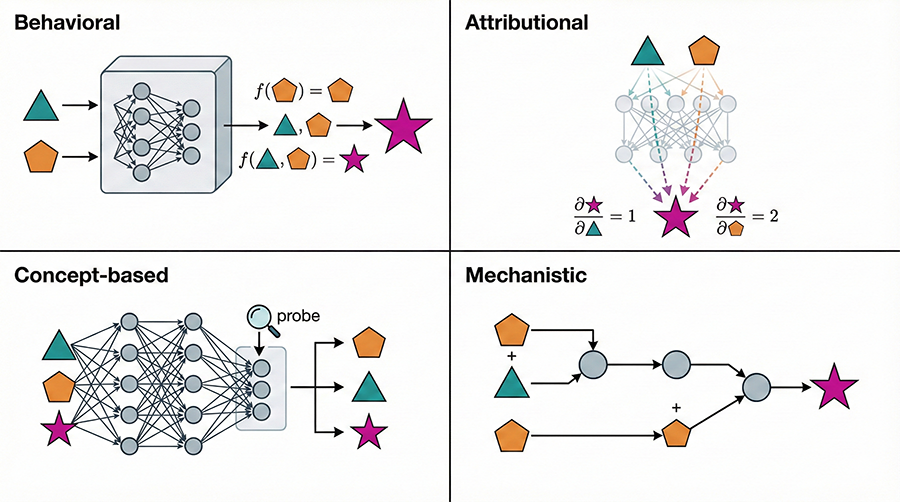
\includegraphics[width=0.96\linewidth]{figures/MI-concepts.png}};
  \begin{scope}[x={(miimage.south east)},y={(miimage.north west)}]
    \fill[white] (0.012,0.923) rectangle (0.488,0.995);
    \fill[white] (0.512,0.923) rectangle (0.990,0.995);
    \fill[white] (0.012,0.418) rectangle (0.488,0.495);
    \fill[white] (0.512,0.418) rectangle (0.990,0.495);
    \node[anchor=north west, font=\small\sffamily\bfseries] at (0.015,0.982) {行为可解释性};
    \node[anchor=north west, font=\small\sffamily\bfseries] at (0.515,0.982) {归因可解释性};
    \node[anchor=north west, font=\small\sffamily\bfseries] at (0.015,0.476) {基于概念的可解释性};
    \node[anchor=north west, font=\small\sffamily\bfseries] at (0.515,0.476) {机制可解释性};
    \fill[white] (0.305,0.348) rectangle (0.367,0.385);
    \node[anchor=west, font=\footnotesize\sffamily] at (0.304,0.367) {探针};
  \end{scope}
\end{tikzpicture}
